\documentclass[12pt]{article}
\usepackage[english]{babel}
\usepackage{graphicx, color, xcolor, wrapfig, subcaption}
\usepackage{amsmath}
\usepackage{hyperref}


%\usepackage{tabularx}
\usepackage{booktabs}

\graphicspath{ {images/} }
\hypersetup{
    colorlinks,%
    citecolor=green,%
    filecolor=magenta,%
    linkcolor=red,%
    urlcolor=cyan
}

\title{CS531 Programming Assignment 1: Vacuum-Cleaning Agents}
\author{
        Santosh Kumar, Daniel Magee \\
        (EECS, MIME), Oregon State University\\
}

\DeclareMathOperator*{\argmin}{arg\,min}
\DeclareMathOperator*{\argmax}{arg\,max}

\begin{document}

\maketitle

\begin{abstract}
In this project, we examine the effectiveness of three types of simple autonomous vacuum agents in two different types of environments. 
To compare the effectiveness of the agents, we consider the number of squares cleaned in the number of moves taken as the performance metric.
We find that the random agent performed well enough to complete the course in both conditions, the simple reflex model could not complete the course, and the deterministic model could complete the open course very well but struggled on the partitioned course.
\end{abstract}

\section{Introduction}

We consider three types of agents in the design of an autonomous vacuum cleaner: a simple reflex agent without persistent memory, a similarly memoryless reflex agent with randomized responses to stimuli, and a model-based agent with a small amount of short term memory.  
Our evaluation of the three designs is based on a simple performance metric: cleaning more cells in fewer movements is preferable.

Each agent is equipped with sensors which gather three percepts from the environment: whether there is dirt in the current cell, whether there is a wall in front of the vacuum and whether the vacuum is in the cell it started in.  
With this information it can take one of five actions: move forward, turn off, pick up the dirt, or turn (left or right).




\section{Algorithms}

\subsection{Memoryless Agent}

The rules for the memory agent are as follows:
\begin{verbatim}
if there is DIRT then SUCK it up 
if there is not DIRT and no WALL and then move FORWARD
if there is not DIRT and a WALL and I am not HOME turn RIGHT
if there is not DIRT and a WALL and I am HOME TURN OFF
\end{verbatim}

The best possible performance for this agent is that it will pick up the dirt in every cell that abuts a wall.
It may also pick up dirt on cells in the field of the room if there are posts staggered so it may run into them and turn without running along a wall.
This experiment does not include this condition so, since it can only turn in corners, it only moves along walls.

\subsection{Random Agent}

The random agent allows for the vacuum to turn even when it is not impeded by an obstacle.
A stochastic distribution is applied to the response function such that the vacuum may turn right or left based on a random choice when confronted with a wall, and may choose to turn when there is no obstacle.
Moving forward when possible is generally the best decision so that choice is heavily weighted.

\subsection{Memory Capable Agent}

\section{Results}

\begin{figure}[!h]
	\centering
	\begin{subfigure}[t]{.48\textwidth}
		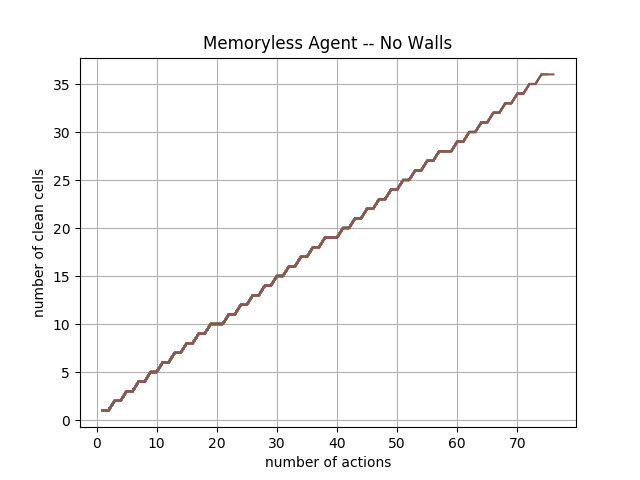
\includegraphics[scale=.4]{MemorylessAgent1}
		\label{fig:MemoryLNoWall}
	\end{subfigure}
	\hfill
	\begin{subfigure}[t]{.48\textwidth}
		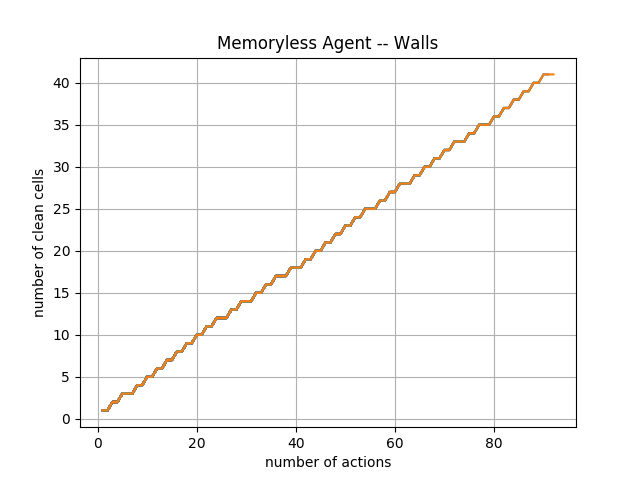
\includegraphics[scale=.4]{MemorylessAgent2}
		\label{fig:MemoryLWall}
	\end{subfigure}
	\caption{The Memoryless agent returns home before all the cells are clean.  It runs in a loop dependent on the room configuration.}
	\label{f:Memoryless}	
\end{figure}

The random agent performs better when there are no obstructions on
average as it would be difficult for it to come back to the initial
position and hence keeps on moving even after cleaning majority of the
cells.

Fine-tuning the parameters, such as stop etc which can improve
performance; as the agent stops after more or less squares are empty. 
Otherwise the number of moves keep on increasing if it doesn’t stop and
performance diminishes, probability of stopping can be increased to
increase performance.

The random agent performs best when it has the space between obstacles to exercise its randomness and explore otherwise unreachable areas of the map.
More constrained areas cause a much larger deviation in the performance of the random agent which is interesting as shown in~\ref{tab:Random}.  
While in overall performance, the random agent takes 50\% longer to clean 90\% of the squares on the walled map, the deviation in the time to clean that area roughly triples.  

\begin{figure}[!h]
	\centering
	\begin{subfigure}[t]{.48\textwidth}
		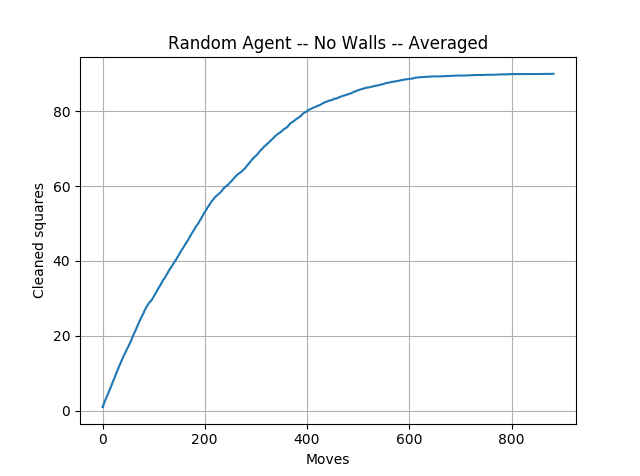
\includegraphics[scale=.4]{RandomAgent1Mean}
		\label{fig:RandomNoWall}
	\end{subfigure}
	\hfill
	\begin{subfigure}[t]{.48\textwidth}
		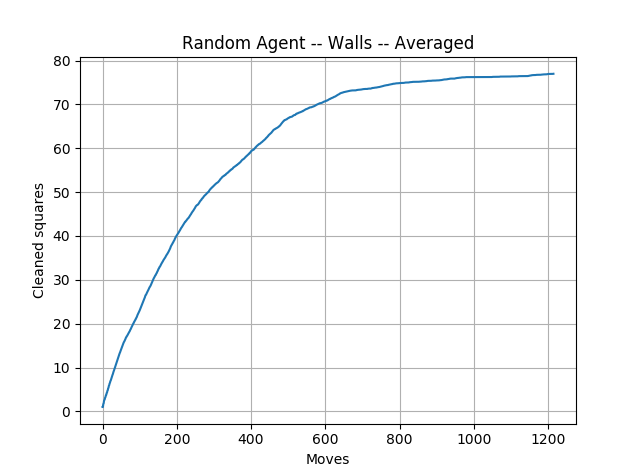
\includegraphics[scale=.4]{RandomAgent2Mean}
		\label{fig:RandomWall}
	\end{subfigure}
	\caption{Averages of the results of the reflex agent with a random component}
	\label{f:Randomless}	
\end{figure}

The agent with memory performs by far the best on the open map~\ref{fig:MemoryFNoWall}.

\begin{figure}[!h]
	\centering
	\begin{subfigure}[t]{.48\textwidth}
		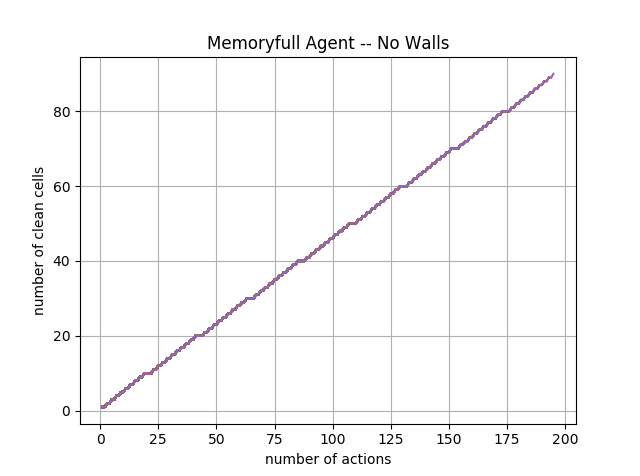
\includegraphics[scale=.4]{MemoryFullAgent1}
		\label{fig:MemoryFNoWall}
	\end{subfigure}
	\hfill
	\begin{subfigure}[t]{.48\textwidth}
		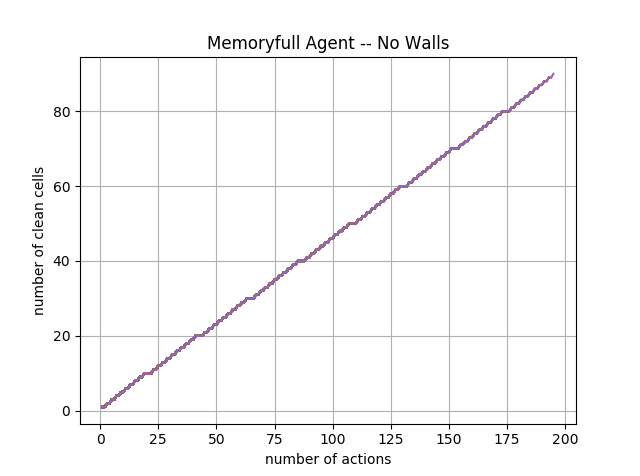
\includegraphics[scale=.4]{MemoryFullAgent1}
		\label{fig:MemoryWall}
	\end{subfigure}
	\caption{The agent capable of deciding movements based on recent actions}
	\label{f:Randomless}	
\end{figure}

\section{Conclusions}
We observe several trade offs between random and deterministic agents.
Deterministic agents have to store a lot of memory which is not
necessary in case of randomized agents.
Randomized agents do not perform well always, they only perform
better on average than simple reflex agents.
Randomness can be useful in cases where there are not many
obstructions or else more steps taken causally without achieving
desired result and the performance diminishes.
Deterministic agents can be good in areas where there are lots of
obstructions because storing state can be useful to avoid pitfalls in
such cases, but they can also get stuck in an area if they don't have enough memory and if the target is in the starting area they may move toward it without completing the course.

If there are polygonal obstacles, we would consider implementing a mix of
random and deterministic memory models where the randomness can help us
deviate away from the object. The model would store such memory to repeat
that path and hence steer away from the polygonal obstacle.

We were surprised that the random agent performed so well, in particular on more closed maps, and that the deterministic model performed so poorly.
Using a different deterministic model, one that suited the particularities of the map would be most beneficial.
We learned that more complexity does not always lead to better results, and that randomness can guide an object as well as a considered algorithm some of the time.

\newpage

\begin{table}
\vspace{-5em}
\caption{Turn Random Agent cleans 90\% of area.}
\vspace{-1.5em}
\label{tab:Random}
\begin{center}
	\footnotesize
\begin{tabular}{lrr}
\toprule
Run &  No Walls &  Walls \\
\midrule
0  &       483 &    783 \\
1  &       767 &    755 \\
2  &       457 &    628 \\
3  &       559 &    641 \\
4  &       667 &    395 \\
5  &       604 &   1050 \\
6  &       643 &   1115 \\
7  &       499 &   1045 \\
8  &       524 &    600 \\
9  &       634 &    670 \\
10 &       536 &   1153 \\
11 &       493 &    677 \\
12 &       465 &    743 \\
13 &       716 &    522 \\
14 &       680 &   1288 \\
15 &       550 &    658 \\
16 &       549 &    572 \\
17 &       548 &   1280 \\
18 &       375 &    472 \\
19 &       620 &    532 \\
20 &       484 &    720 \\
21 &       554 &   1140 \\
22 &       480 &    479 \\
23 &       574 &    510 \\
24 &       521 &   1440 \\
25 &       543 &    525 \\
26 &       423 &    441 \\
27 &       685 &    686 \\
28 &       404 &    849 \\
29 &       463 &   1173 \\
30 &       688 &    589 \\
31 &       569 &    511 \\
32 &       643 &    930 \\
33 &       649 &    648 \\
34 &       723 &   1046 \\
35 &       598 &   1059 \\
36 &       554 &    828 \\
37 &       464 &    941 \\
38 &       499 &    760 \\
39 &       567 &    709 \\
40 &       519 &    590 \\
41 &       582 &    651 \\
42 &       541 &   1184 \\
43 &       659 &    771 \\
44 &       566 &    561 \\
45 &       350 &    753 \\
46 &       330 &    687 \\
47 &       490 &    789 \\
48 &       522 &    443 \\
49 &       488 &    694 \\ 
\textbf{mean} & \textbf{550.02} & \textbf{773.72} \\
\textbf{stdev} & \textbf{96.01}  & \textbf{256.95} \\
\bottomrule
\end{tabular}
\end{center}
\end{table}


\end{document}